
\documentclass[11pt]{article}
\usepackage[margin=1in]{geometry}

% Core packages
\usepackage{amsmath,amssymb}
\usepackage{tikz-cd}
\usetikzlibrary{arrows.meta,positioning,fit,backgrounds}
\usepackage{multicol}
\usepackage{graphicx}
\usepackage{array}
\usepackage{tabularx}
\usepackage{longtable}
\usepackage{enumitem}
\usepackage{listings}

\lstset{
    basicstyle=\ttfamily\footnotesize,
    breaklines=true,
    columns=fullflexible,
    frame=single,
    showstringspaces=false,
    tabsize=2
}

\newcommand{\apiendpoint}[1]{\texttt{\detokenize{#1}}}

% Paragraphs
\setlength{\parindent}{0pt}
\setlength{\parskip}{1\baselineskip}
\setlist[itemize]{itemsep=0.25em,topsep=0.4em}

\begin{document}

\begin{titlepage}
    \thispagestyle{empty}
    \centering
    \vspace*{0.20\textheight}

    {\Huge\bfseries Workforce Execution Platform\par}

    \vspace{0.8cm}
    \rule{0.72\textwidth}{0.8pt}\par
    \vspace{0.8cm}

    {\LARGE Solution Architecture Proposal\par}

    \vfill

    {\large
    \textbf{Prepared by:}\par
    \vspace{0.3cm}
    Ali Almanea\par

    \vspace{1.2cm}

    \textbf{Date:}\par
    \vspace{0.3cm}
    23 July 2026\par
    }

    \vspace*{0.10\textheight}
\end{titlepage}

\tableofcontents
\clearpage

\section{Introduction}

The current workforce execution process relies on Excel spreadsheets,
paper-based forms, and manual approval procedures. These disconnected processes
make daily planning, workforce assignment, execution tracking, and reporting
inefficient, error-prone, and difficult to monitor in real time.

This document proposes a Minimum Viable Product (MVP) solution for a Workforce
Execution Platform that digitizes the end-to-end daily execution lifecycle. The
proposed solution enables Technical Office Engineers to create daily work plans,
Heads of Master to manage field execution and workforce assignments, and
management to review, approve, and monitor operational progress through a
centralized platform.

The proposed architecture follows a modular, layered design that prioritizes
maintainability, security, and scalability while keeping the MVP implementation
simple. The solution is also designed to support future business expansion,
including configurable workflows, additional approval levels, and advanced
reporting capabilities, without requiring major architectural changes.

\section{Business Process Overview}

The Workforce Execution Platform digitizes the complete daily field execution
process, replacing Excel spreadsheets, paper forms, and manual approvals with a
centralized workflow. The platform manages Daily Planning, Crew Assignment,
Work Execution, the Approval Workflow, and Daily Reporting within a single
coordinated process. This end-to-end flow gives business stakeholders,
architects, and developers a shared view of how planned work progresses from
the monthly production plan to operational dashboards and KPI reporting.

\subsection{Business Process Diagram}

\begin{figure}[htbp]
    \centering
    \begin{tikzcd}[column sep=0.55cm, row sep=0.65cm, cells={nodes={draw,
        rounded corners, align=center, minimum height=1.25cm,
        text width=0.18\textwidth, font=\small}}]
        \text{\shortstack{Monthly\\Production Plan}}
        \arrow[r] &
        \text{\shortstack{Technical Office\\Creates Daily Plan}}
        \arrow[r] &
        \text{\shortstack{Assign Work to\\Head of Master}}
        \arrow[r] &
        \text{\shortstack{Head of Master\\Creates Crew\\Assigns Workers}}
        \arrow[d] \\
        \text{\shortstack{Project Manager\\Approval}}
        \arrow[d] &
        \text{\shortstack{Site Chief\\Review}}
        \arrow[l] &
        \text{\shortstack{Submit Actual\\Quantity\\Man-Day\\Overtime\\Comments}}
        \arrow[l] &
        \text{\shortstack{Execute Daily\\Work}}
        \arrow[l] \\
        \text{Daily Report}
        \arrow[r] &
        \text{\shortstack{Power BI\\Dashboard}}
    \end{tikzcd}
    \caption{End-to-End Business Process of the Workforce Execution Platform}
    \label{fig:business-process-overview}
\end{figure}

\subsection{Business Flow Explanation}

\begin{enumerate}
    \item The Monthly Production Plan provides the source for daily planning.
    \item The Technical Office creates Daily Plans from the planned activities.
    \item Daily Plans are assigned to the responsible Head of Master.
    \item The Head of Master creates crews and assigns workers.
    \item Workers execute the planned activities.
    \item At the end of the day, actual quantity, Man-Day, overtime, and comments
          are submitted.
    \item The Site Chief reviews the submission.
    \item The Project Manager performs the final approval.
    \item Approved records are automatically consolidated into Daily Reports.
    \item Power BI provides operational dashboards and KPI reporting.
\end{enumerate}

\section{Assumptions}

Since the case study does not explicitly define all business rules, the
following assumptions have been made for the MVP solution:

\begin{itemize}
    \item A project may contain multiple Regions.
    \item Each Region may contain multiple Locations (KKK).
    \item Each Location is assigned to a single Head of Master.
    \item A Head of Master may manage one or more Locations.
    \item Each Region has one Technical Office Engineer responsible for creating
          Daily Plans.
    \item Each Region has one Site Chief responsible for reviewing submitted
          work.
    \item Each Project has one Project Manager responsible for final approval.
    \item A Daily Plan belongs to a single Project, Region, and Location.
    \item The approval workflow is fixed in the MVP: Technical Office
          $\rightarrow$ Head of Master $\rightarrow$ Site Chief
          $\rightarrow$ Project Manager.
    \item Authentication is managed internally using Role-Based Access Control
          (RBAC).
    \item Mobile devices may temporarily lose network connectivity; therefore,
          offline synchronization is required.
    \item Approved Daily Plans are automatically consolidated into the Daily
          Report and become available for Power BI reporting.
\end{itemize}

\section{Functional Requirements}

\subsection{Daily Planning}

\begin{itemize}
    \item Technical Office Engineers shall be able to create Daily Plans based
          on the monthly production plan.
    \item The system shall allow the selection of Project, ToW, SToW, and
          SSToW.
    \item Planned Quantity and Planned Man-Day values shall be recorded.
    \item Daily Plans shall be assigned to the appropriate Head of Master.
\end{itemize}

\subsection{Crew Management}

\begin{itemize}
    \item Heads of Master shall be able to view assigned Daily Plans.
    \item Heads of Master shall create crews based on worker types.
    \item Workers shall be assigned to crews.
    \item Assigned work shall be started and managed through the mobile
          application.
\end{itemize}

\subsection{Execution Reporting}

\begin{itemize}
    \item Heads of Master shall record Actual Quantity.
    \item Heads of Master shall record Actual Man-Day.
    \item Overtime information shall be recorded.
    \item Comments shall be mandatory when work is partially completed or not
          started.
    \item Additional execution details (ZZZ) shall be captured where required.
\end{itemize}

\subsection{Approval Workflow}

\begin{itemize}
    \item Submitted Daily Plans shall be reviewed by the Site Chief.
    \item Approved records shall proceed to the Project Manager.
    \item Rejected records shall require a mandatory rejection reason.
    \item The responsible Head of Master shall be notified when a Daily Plan is
          rejected.
    \item Corrected Daily Plans may be resubmitted for approval.
\end{itemize}

\subsection{Reporting}

\begin{itemize}
    \item Approved Daily Plans shall be automatically consolidated into a Daily
          Report.
    \item Operational KPIs shall be available through Power BI.
    \item Reports shall include:
          \begin{itemize}
              \item Planned vs. Actual Quantity
              \item Productivity
              \item Man-Day
              \item Overtime
          \end{itemize}
\end{itemize}

\subsection{Authentication \& Authorization}

\begin{itemize}
    \item Users shall authenticate securely before accessing the platform.
    \item Access shall be controlled using Role-Based Access Control (RBAC).
    \item Permissions shall be assigned based on business responsibilities.
    \item Users shall only access resources within their authorized Project,
          Region, or Location scope.
\end{itemize}

\subsection{Notifications}

\begin{itemize}
    \item Heads of Master shall receive notifications when new Daily Plans are
          assigned.
    \item Site Chiefs shall be notified when a Daily Plan is submitted.
    \item Project Managers shall receive notifications after Site Chief
          approval.
    \item Users shall receive notifications when a Daily Plan is rejected or
          requires further action.
\end{itemize}

\section{Non-Functional Requirements}

\renewcommand{\arraystretch}{1.25}
\begin{tabularx}{\textwidth}{|>{\raggedright\arraybackslash}p{0.20\textwidth}|>{\raggedright\arraybackslash}X|}
    \hline
    \textbf{Requirement} & \textbf{Description} \\
    \hline
    Scalability & The architecture shall support future expansion to additional
    projects, regions, locations, users, and business workflows without major
    redesign. \\
    \hline
    Performance & Common API operations should respond quickly under normal
    operational load. \\
    \hline
    Availability & The platform should remain available during normal
    infrastructure failures and support high operational uptime. \\
    \hline
    Offline Support & Mobile users shall continue working without internet
    connectivity. Changes shall be synchronized automatically once connectivity
    is restored. \\
    \hline
    Security & The system shall enforce secure authentication, authorization,
    encrypted communication (HTTPS), password hashing, and audit logging. \\
    \hline
    Maintainability & The solution shall follow a layered architecture with
    clear separation of concerns to simplify future maintenance. \\
    \hline
    Extensibility & New approval stages, permissions, reports, and business
    rules shall be added with minimal impact on the existing architecture. \\
    \hline
    Reliability & Data consistency shall be maintained throughout the approval
    workflow, preventing duplicate submissions and invalid state transitions. \\
    \hline
    Auditability & Critical business actions (creation, updates, approvals, and
    rejections) shall be recorded for traceability. \\
    \hline
\end{tabularx}
\renewcommand{\arraystretch}{1}

\clearpage
\section{High-Level Architecture}

The proposed solution follows a Modular Monolith Architecture, which provides a
simple deployment model while maintaining clear separation between business
capabilities. This approach is well suited for the MVP phase, reducing
operational complexity while allowing future modularization if business
requirements grow.

\begin{figure}[htbp]
    \centering
    \includegraphics[width=0.88\textwidth]{prism-uploads/exact_copy_architecture.png}
    \caption{High-level architecture of the Workforce Execution Platform.}
    \label{fig:high-level-architecture}
\end{figure}

The architecture consists of four primary layers:

\begin{itemize}
    \item \textbf{Client Layer:} A desktop web application is used by Technical Office
          Engineers, Site Chiefs, and Project Managers, while Heads of Master
          interact with the system through a mobile application.

    \item \textbf{Application Layer:} A single backend application exposes REST APIs
          and contains all business modules, including Daily Planning, Crew
          Management, Approval Workflow, Reporting, Notifications, and Audit.
          Authentication is handled using JWT, while authorization is enforced
          through Role-Based Access Control (RBAC), permission-based
          authorization, and Project/Region/Location scope validation.

    \item \textbf{Data Layer:} PostgreSQL serves as the primary system of record for
          operational data, workflow states, and audit history. Redis is used to
          cache permissions and frequently accessed reference data, improving
          application performance.

    \item \textbf{External Services:} Power BI connects directly to PostgreSQL using
          read-only access to generate dashboards and KPI reports. Push
          notifications are delivered through Firebase Cloud Messaging (FCM)
          to notify Heads of Master about new assignments, approvals, and
          workflow updates.
\end{itemize}

\subsection{Redis Cache}

Redis stores short-lived or frequently requested data that can be safely
reconstructed from PostgreSQL:

\begin{itemize}
    \item \textbf{User Sessions:} Active session metadata, refresh-token
          references, and session-expiration information.
    \item \textbf{Permission Cache:} The effective permissions resolved for an
          authenticated user.
    \item \textbf{Role Cache:} User-to-role assignments and the permissions
          associated with each role.
    \item \textbf{Frequently Accessed Master Data:} Stable reference data such
          as Projects, Regions, Locations, and work-classification values.
\end{itemize}

Caching this information reduces repeated database queries and improves API
response time while PostgreSQL remains the authoritative system of record.

A typical request starts from either the desktop or mobile application, reaches
the backend through secure REST APIs, passes authentication and authorization
checks, and is processed by the corresponding business module. Business data is
persisted in PostgreSQL, while notification events are forwarded to Firebase
Cloud Messaging for delivery to mobile users. Reporting data is consumed
directly by Power BI without affecting transactional operations.

\clearpage
\section{Layered Architecture}

The backend is organized into distinct layers, with each layer having a focused
responsibility. Requests move inward from the user interface toward the business
rules, while infrastructure details remain isolated from the core application
logic. This separation improves maintainability, testability, and the ability to
replace technical components without changing business behavior.

\begin{figure}[htbp]
    \centering
    \includegraphics[width=0.82\textwidth]{prism-uploads/layered_architecture.png}
    \caption{Layered architecture and dependency flow.}
    \label{fig:layered-architecture}
\end{figure}

The architecture is divided into the following layers:

\begin{itemize}
    \item \textbf{Presentation Layer:} Contains the desktop web application and
          mobile application through which users interact with the platform.

    \item \textbf{API/Controllers Layer:} Exposes REST endpoints, validates
          incoming requests, verifies JWT access tokens, and forwards authorized
          operations to the application layer.

    \item \textbf{Application Layer:} Coordinates business use cases such as
          daily planning, crew management, execution reporting, approvals, and
          notifications. It manages application workflows without containing
          infrastructure-specific implementation details.

    \item \textbf{Domain Layer:} Contains the core domain entities, business
          rules, project-scope rules, RBAC policies, and workflow invariants.
          This layer represents the central business model of the platform.

    \item \textbf{Infrastructure Layer:} Implements database repositories, data
          adapters, cache integrations, and external-service clients required by
          the application and domain layers.

    \item \textbf{External Services and Persistence:} PostgreSQL stores
          operational and audit data, Redis provides caching, Firebase Cloud
          Messaging delivers mobile notifications, and Power BI consumes data
          through read-only analytics access.
\end{itemize}

Dependencies flow from the outer layers toward the application and domain
layers. The domain model remains independent of presentation, database, cache,
and notification technologies, allowing these components to be tested or
replaced with minimal impact on the core business rules.

\clearpage
\begingroup
\setlength{\parskip}{0.45\baselineskip}
\section{Domain Model \& Workflow}

\subsection{Workflow Overview}

The Workforce Execution Platform follows a predefined approval workflow that
reflects the current business process. Each Daily Plan progresses through a
series of workflow states. Every state transition requires specific business
validations and appropriate user permissions.

For the MVP, the workflow is implemented as a fixed state machine within the
application. However, the design intentionally separates workflow logic from
business modules, allowing future migration to a configuration-driven workflow
engine without significant architectural changes.

The workflow is illustrated below.

\begin{figure}[htbp]
    \centering
    \includegraphics[height=0.52\textheight,keepaspectratio]{prism-uploads/advanced_workflow_3.png}
    \caption{Daily Plan approval workflow, including rejection and resubmission.}
    \label{fig:advanced-workflow}
\end{figure}

\clearpage
\subsection{Workflow States}

\renewcommand{\arraystretch}{1.05}
\scriptsize
\begin{tabularx}{\textwidth}{|>{\raggedright\arraybackslash}p{0.17\textwidth}|>{\raggedright\arraybackslash}X|>{\raggedright\arraybackslash}p{0.18\textwidth}|>{\raggedright\arraybackslash}p{0.24\textwidth}|}
    \hline
    \textbf{Status} & \textbf{Description} & \textbf{Responsible Role} &
    \textbf{Required Permission} \\
    \hline
    Draft & Daily Plan is created by Technical Office. & Technical Office
    Engineer & \texttt{daily\_plan.\allowbreak create} \\
    \hline
    Assigned & Daily Plan is assigned to a Head of Master. & Technical Office
    Engineer & \texttt{daily\_plan.\allowbreak assign} \\
    \hline
    In Progress & Crew is created and field execution starts. & Head of Master &
    \texttt{daily\_plan.\allowbreak start\_execution} \\
    \hline
    Submitted & Actual Quantity, Man-Day, Overtime, and comments are submitted.
    & Head of Master & \texttt{daily\_plan.\allowbreak submit} \\
    \hline
    Rejected & Plan requires corrections before approval. & Site Chief / Project
    Manager & \texttt{daily\_plan.\allowbreak reject} \\
    \hline
    Approved by Site Chief & Daily Plan approved by Site Chief. & Site Chief &
    \texttt{daily\_plan.\allowbreak approve.\allowbreak site\_chief} \\
    \hline
    Approved by Project Manager & Final business approval. & Project Manager &
    \texttt{daily\_plan.\allowbreak approve.\allowbreak project\_manager} \\
    \hline
    Completed & Workflow finished successfully. & System & --- \\
    \hline
\end{tabularx}
\renewcommand{\arraystretch}{1}

\subsection{Transition Rules}

\renewcommand{\arraystretch}{1.05}
\begin{tabularx}{\textwidth}{|>{\raggedright\arraybackslash}p{0.38\textwidth}|>{\raggedright\arraybackslash}X|}
    \hline
    \textbf{Current Status} & \textbf{Next Status} \\
    \hline
    Draft & Assigned \\
    \hline
    Assigned & In Progress \\
    \hline
    In Progress & Submitted \\
    \hline
    Submitted & Approved by Site Chief, Rejected \\
    \hline
    Rejected & Submitted \\
    \hline
    Approved by Site Chief & Approved by Project Manager, Rejected \\
    \hline
    Approved by Project Manager & Completed \\
    \hline
\end{tabularx}
\renewcommand{\arraystretch}{1}

In the MVP state model, resubmission is the action that moves a rejected record
back to the Submitted state rather than a separately persisted status.

\normalsize
\clearpage
\subsection{MVP Workflow Design}

For the MVP, workflow states and transitions are implemented directly in the
application to minimize complexity and accelerate development.

Although the workflow is fixed, the architecture is designed to support a
future configuration-driven workflow engine. This approach allows business
administrators to modify approval stages, permissions, and transition rules
without changing application code.

A future configuration may resemble the following JSON structure.

\begin{lstlisting}[basicstyle=\ttfamily\scriptsize]
{
  "Draft": {
    "allowedTransitions": ["Assigned"],
    "requiredPermission": "daily_plan.assign",
    "validators": ["ProjectSelected", "LocationSelected",
      "QuantityEntered", "HeadOfMasterAssigned"]
  },
  "Assigned": {
    "allowedTransitions": ["InProgress"],
    "requiredPermission": "daily_plan.start_execution",
    "validators": ["CrewCreated", "WorkersAssigned"]
  },
  "InProgress": {
    "allowedTransitions": ["Submitted"],
    "requiredPermission": "daily_plan.submit",
    "validators": ["ActualQuantityEntered",
      "ActualManDayEntered"]
  },
  "Submitted": {
    "allowedTransitions": ["ApprovedBySiteChief", "Rejected"],
    "requiredPermission": "daily_plan.approve.site_chief",
    "validators": ["SubmissionCompleted"],
    "actions": ["NotifySiteChief", "CreateAuditRecord"]
  },
  "Rejected": {
    "allowedTransitions": ["Submitted"],
    "requiredPermission": "daily_plan.resubmit",
    "validators": ["RejectionCommentProvided"]
  },
  "ApprovedBySiteChief": {
    "allowedTransitions": ["ApprovedByProjectManager", "Rejected"],
    "requiredPermission": "daily_plan.approve.project_manager",
    "validators": ["SiteChiefApprovalCompleted"],
    "actions": ["NotifyProjectManager"]
  },
  "ApprovedByProjectManager": {
    "allowedTransitions": ["Completed"],
    "requiredPermission": "daily_plan.complete",
    "validators": []
  },
  "Completed": {
    "allowedTransitions": [],
    "requiredPermission": null,
    "validators": []
  }
}
\end{lstlisting}

\endgroup

\clearpage
\section{Data Model (ER Diagram)}

\subsection{Overview}

The database is designed following a normalized relational model to support the
Workforce Execution Platform MVP. The model separates identity management,
organizational structure, operational planning, workflow tracking, and
notifications into independent entities to improve maintainability and future
scalability.

The design aims to minimize data duplication while preserving clear
relationships between projects, organizational units, users, and daily
execution activities.

The data model is organized into the following logical domains:

\begin{itemize}
    \item \textbf{Identity \& Authorization:} Manages users, roles, permissions,
          and access scopes.
    \item \textbf{Organization Structure:} Represents Projects, Regions, and
          Locations.
    \item \textbf{Work Breakdown Structure (WBS):} Models ToW, SToW, and SSToW
          hierarchies.
    \item \textbf{Planning \& Execution:} Stores Daily Plans, crew information,
          and assigned workers.
    \item \textbf{Workflow:} Records status transitions and approval history.
    \item \textbf{Notifications:} Stores in-app notification records for users.
\end{itemize}

\begin{figure}[htbp]
    \centering
    \includegraphics[width=\textwidth,height=0.84\textheight,keepaspectratio]{prism-uploads/final_verified_er_2.png}
    \caption{Entity relationship diagram for the Workforce Execution Platform MVP.}
    \label{fig:data-model-er}
\end{figure}

\clearpage
\subsection{Authorization Database Model (DBML)}

The authorization portion of the database model retains the existing
\texttt{user\_scopes} table and makes role assignments project-specific through
\texttt{user\_roles.project\_id}. The relevant DBML definition is shown below.

\begin{lstlisting}[basicstyle=\ttfamily\scriptsize]
Table users {
  id uuid [pk]
  full_name varchar
  email varchar [unique, not null]
  password_hash varchar [not null]
  is_active boolean [not null]
}

Table projects {
  id uuid [pk]
  name varchar [not null]
  code varchar [unique, not null]
}

Table regions {
  id uuid [pk]
  project_id uuid [not null, ref: > projects.id]
  name varchar [not null]
}

Table locations {
  id uuid [pk]
  region_id uuid [not null, ref: > regions.id]
  code varchar [unique, not null]
  name varchar [not null]
}

Table roles {
  id uuid [pk]
  name varchar [unique, not null]
}

Table permissions {
  id uuid [pk]
  code varchar [unique, not null]
  description varchar
}

Table user_roles {
  user_id uuid [not null, ref: > users.id]
  project_id uuid [not null, ref: > projects.id]
  role_id uuid [not null, ref: > roles.id]

  indexes {
    (user_id, project_id, role_id) [unique]
  }
}

Table role_permissions {
  role_id uuid [not null, ref: > roles.id]
  permission_id uuid [not null, ref: > permissions.id]

  indexes {
    (role_id, permission_id) [unique]
  }
}

Table user_scopes {
  id uuid [pk]
  user_id uuid [not null, ref: > users.id]
  project_id uuid [not null, ref: > projects.id]
  region_id uuid [ref: > regions.id]
  location_id uuid [ref: > locations.id]
}
\end{lstlisting}

\subsection{Design Decisions}

The following design decisions were made while modeling the database:

\begin{itemize}
    \item Each \textbf{Daily Plan} belongs to a single Project, Region, and
          Location.
    \item A Daily Plan references one ToW, one SToW, and one SSToW according to
          the Work Breakdown Structure.
    \item A Technical Office Engineer creates the Daily Plan and assigns it to a
          Head of Master responsible for field execution.
    \item A Crew is created for each Daily Plan and may contain multiple
          workers.
    \item Workers are modeled as business entities rather than application
          users, since the case study does not specify that workers directly
          access the system.
    \item Workflow history is stored separately from the current Daily Plan
          state to provide a complete audit trail of approvals, rejections, and
          status changes.
    \item User permissions are managed using Role-Based Access Control (RBAC),
          while Project, Region, and Location access is enforced through scope
          assignments.
    \item User roles are assigned per Project through the
          \texttt{user\_roles} table. Its composite unique constraint on
          \texttt{(user\_id, project\_id, role\_id)} prevents the same role from
          being assigned to the same user more than once within a Project while
          allowing different assignments across Projects.
    \item The existing \texttt{user\_scopes} model is retained to represent
          Project, Region, and Location access; no separate user-assignment
          model is required for the MVP.
    \item Conflicting operational roles are not enforced through database
          constraints. The backend validates Separation of Duties rules before
          creating or changing a Project role assignment.
\end{itemize}

\subsection{Entity Relationships}

The main relationships within the data model are summarized below:

\begin{itemize}
    \item A \textbf{Project} contains multiple Regions.
    \item A \textbf{Region} contains multiple Locations.
    \item A \textbf{Location} may contain multiple Daily Plans.
    \item A \textbf{Daily Plan} belongs to exactly one Project, Region, and
          Location.
    \item A \textbf{Daily Plan} is assigned to one Head of Master.
    \item A \textbf{Crew} belongs to one Daily Plan.
    \item A \textbf{Crew} may contain multiple workers.
    \item A \textbf{Worker} may participate in multiple crews over time.
    \item Every workflow transition is recorded in the \textbf{Workflow
          History} table.
    \item Notifications are linked to the target application user.
    \item A \textbf{User Role} links one User, one Project, and one Role.
    \item A \textbf{Role} is linked to its Permissions through
          \textbf{Role Permissions}.
    \item A \textbf{User Scope} links a User to an authorized Project and,
          where applicable, a Region or Location within that Project.
\end{itemize}

\subsection{MVP Considerations}

For the MVP, the database model intentionally favors simplicity while remaining
extensible.

Several business concepts, such as workflow definitions, approval
configurations, and dynamic business rules, are implemented directly in the
application layer rather than being stored as configurable database entities.

This approach reduces implementation complexity during the MVP phase while
allowing future migration toward a configuration-driven workflow engine without
significant database redesign.

The database prevents duplicate Project role assignments through the composite
unique constraint. Business conflicts remain application rules: a user cannot
hold more than one operational role---Head of Master, Site Chief, Technical
Office Engineer, or Project Manager---within the same Project.

\clearpage
\section{REST API Design}

\subsection{API Design Principles}

The Workforce Execution Platform exposes a RESTful API that serves both the
desktop web application and the mobile application. All clients communicate
with the same API, ensuring consistent business rules and centralized
authorization.

The API follows these design principles:

\begin{itemize}
    \item RESTful, resource-oriented endpoints.
    \item A versioned API (\apiendpoint{/api/v1}) to support future evolution.
    \item JWT-based authentication.
    \item Role-Based Access Control (RBAC) and permission validation for every
          protected endpoint.
    \item Project, Region, and Location scope validation.
    \item Consistent request and response formats.
    \item Standard HTTP status codes.
    \item Pagination, filtering, and sorting for list endpoints.
\end{itemize}

\subsection{Authentication APIs}

\renewcommand{\arraystretch}{1.15}
\small
\begin{tabularx}{\textwidth}{|>{\raggedright\arraybackslash}p{0.12\textwidth}|>{\raggedright\arraybackslash}p{0.46\textwidth}|>{\raggedright\arraybackslash}X|}
    \hline
    \textbf{Method} & \textbf{Endpoint} & \textbf{Description} \\
    \hline
    POST & \apiendpoint{/api/v1/auth/login} & Authenticate user \\
    \hline
    POST & \apiendpoint{/api/v1/auth/refresh} & Refresh JWT token \\
    \hline
    GET & \apiendpoint{/api/v1/users/me} & Get current user profile \\
    \hline
\end{tabularx}
\normalsize
\renewcommand{\arraystretch}{1}

\subsection{Daily Planning APIs}

\renewcommand{\arraystretch}{1.15}
\small
\begin{tabularx}{\textwidth}{|>{\raggedright\arraybackslash}p{0.12\textwidth}|>{\raggedright\arraybackslash}p{0.46\textwidth}|>{\raggedright\arraybackslash}X|}
    \hline
    \textbf{Method} & \textbf{Endpoint} & \textbf{Description} \\
    \hline
    GET & \apiendpoint{/api/v1/daily-plans} & List Daily Plans \\
    \hline
    POST & \apiendpoint{/api/v1/daily-plans} & Create Daily Plan \\
    \hline
    GET & \apiendpoint{/api/v1/daily-plans/{id}} & Get Daily Plan details \\
    \hline
    PUT & \apiendpoint{/api/v1/daily-plans/{id}} & Update Daily Plan \\
    \hline
    DELETE & \apiendpoint{/api/v1/daily-plans/{id}} & Cancel or delete Daily Plan \\
    \hline
    POST & \apiendpoint{/api/v1/daily-plans/{id}/assign} & Assign Head of Master \\
    \hline
\end{tabularx}
\normalsize
\renewcommand{\arraystretch}{1}

\subsection{Crew Management APIs}

\renewcommand{\arraystretch}{1.15}
\small
\begin{tabularx}{\textwidth}{|>{\raggedright\arraybackslash}p{0.12\textwidth}|>{\raggedright\arraybackslash}p{0.46\textwidth}|>{\raggedright\arraybackslash}X|}
    \hline
    \textbf{Method} & \textbf{Endpoint} & \textbf{Description} \\
    \hline
    POST & \apiendpoint{/api/v1/crews} & Create Crew \\
    \hline
    GET & \apiendpoint{/api/v1/crews/{id}} & Get Crew details \\
    \hline
    POST & \apiendpoint{/api/v1/crews/{id}/workers} & Assign Worker \\
    \hline
    DELETE & \apiendpoint{/api/v1/crews/{id}/workers/{workerId}} & Remove Worker \\
    \hline
\end{tabularx}
\normalsize
\renewcommand{\arraystretch}{1}

\subsection{Workflow APIs}

\renewcommand{\arraystretch}{1.15}
\small
\begin{tabularx}{\textwidth}{|>{\raggedright\arraybackslash}p{0.12\textwidth}|>{\raggedright\arraybackslash}p{0.46\textwidth}|>{\raggedright\arraybackslash}X|}
    \hline
    \textbf{Method} & \textbf{Endpoint} & \textbf{Description} \\
    \hline
    POST & \apiendpoint{/api/v1/daily-plans/{id}/start} & Start execution \\
    \hline
    POST & \apiendpoint{/api/v1/daily-plans/{id}/submit} & Submit execution results \\
    \hline
    POST & \apiendpoint{/api/v1/daily-plans/{id}/approve} & Approve current workflow step \\
    \hline
    POST & \apiendpoint{/api/v1/daily-plans/{id}/reject} & Reject current workflow step \\
    \hline
    GET & \apiendpoint{/api/v1/daily-plans/{id}/history} & Retrieve workflow history \\
    \hline
\end{tabularx}
\normalsize
\renewcommand{\arraystretch}{1}

The API intentionally uses one \apiendpoint{/approve} operation rather than
role-specific endpoints such as \apiendpoint{/approve/site-chief} and
\apiendpoint{/approve/project-manager}. The backend evaluates the current workflow
stage and verifies whether the requesting user has the required role,
permission, and organizational scope. This design is cleaner and easier to
extend as approval stages evolve.

\subsection{Notification APIs}

\renewcommand{\arraystretch}{1.15}
\small
\begin{tabularx}{\textwidth}{|>{\raggedright\arraybackslash}p{0.12\textwidth}|>{\raggedright\arraybackslash}p{0.46\textwidth}|>{\raggedright\arraybackslash}X|}
    \hline
    \textbf{Method} & \textbf{Endpoint} & \textbf{Description} \\
    \hline
    GET & \apiendpoint{/api/v1/notifications} & List notifications \\
    \hline
    PATCH & \apiendpoint{/api/v1/notifications/{id}/read} & Mark notification as read \\
    \hline
\end{tabularx}
\normalsize
\renewcommand{\arraystretch}{1}

\begin{figure}[htbp]
    \centering
    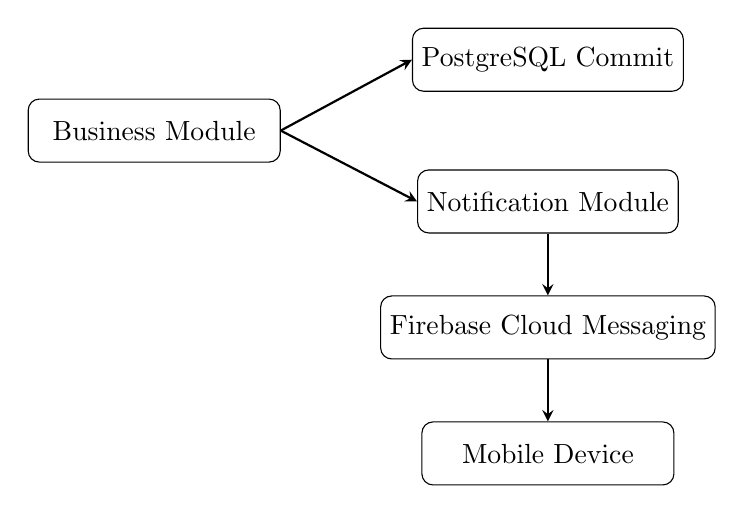
\begin{tikzpicture}[>=stealth]
        \node[draw,rounded corners,align=center,minimum width=3.2cm,
              minimum height=0.8cm] (business) at (0,0) {Business Module};
        \node[draw,rounded corners,align=center,minimum width=3.2cm,
              minimum height=0.8cm] (database) at (5,0.9) {PostgreSQL Commit};
        \node[draw,rounded corners,align=center,minimum width=3.2cm,
              minimum height=0.8cm] (notification) at (5,-0.9)
              {Notification Module};
        \node[draw,rounded corners,align=center,minimum width=3.2cm,
              minimum height=0.8cm] (fcm) at (5,-2.5)
              {Firebase Cloud Messaging};
        \node[draw,rounded corners,align=center,minimum width=3.2cm,
              minimum height=0.8cm] (device) at (5,-4.1) {Mobile Device};

        \draw[->,thick] (business.east) -- (database.west);
        \draw[->,thick] (business.east) -- (notification.west);
        \draw[->,thick] (notification) -- (fcm);
        \draw[->,thick] (fcm) -- (device);
    \end{tikzpicture}
    \caption{Asynchronous notification delivery flow.}
    \label{fig:notification-flow}
\end{figure}

Notification delivery is asynchronous and never blocks the business
transaction.

\subsection{Reporting APIs}

\renewcommand{\arraystretch}{1.15}
\small
\begin{tabularx}{\textwidth}{|>{\raggedright\arraybackslash}p{0.12\textwidth}|>{\raggedright\arraybackslash}p{0.46\textwidth}|>{\raggedright\arraybackslash}X|}
    \hline
    \textbf{Method} & \textbf{Endpoint} & \textbf{Description} \\
    \hline
    GET & \apiendpoint{/api/v1/reports/daily} & Daily operational report \\
    \hline
    GET & \apiendpoint{/api/v1/reports/productivity} & Productivity KPIs \\
    \hline
\end{tabularx}
\normalsize
\renewcommand{\arraystretch}{1}

For the MVP, these APIs display reporting data within the platform. Power BI
uses a separate read-only database connection to produce analytical reports and
dashboards without adding load to transactional API operations.

Power BI connects using read-only access. Reporting never modifies
transactional data. Analytical queries remain isolated from operational
workloads.

\subsection{Standard Response Format}

Successful responses follow a consistent structure:

\begin{lstlisting}[basicstyle=\ttfamily\small]
{
  "success": true,
  "data": {},
  "message": "Operation completed successfully."
}
\end{lstlisting}

Error responses follow the same structure:

\begin{lstlisting}[basicstyle=\ttfamily\small]
{
  "success": false,
  "error": {
    "code": "FORBIDDEN",
    "message": "You do not have permission to perform this action."
  }
}
\end{lstlisting}

\subsection{HTTP Status Codes}

\renewcommand{\arraystretch}{1.15}
\begin{tabularx}{\textwidth}{|>{\raggedright\arraybackslash}p{0.30\textwidth}|>{\raggedright\arraybackslash}X|}
    \hline
    \textbf{Code} & \textbf{Description} \\
    \hline
    200 OK & Successful request \\
    \hline
    201 Created & Resource created successfully \\
    \hline
    204 No Content & Resource deleted successfully \\
    \hline
    400 Bad Request & Validation error \\
    \hline
    401 Unauthorized & Authentication required \\
    \hline
    403 Forbidden & Permission denied \\
    \hline
    404 Not Found & Resource not found \\
    \hline
    409 Conflict & Business rule conflict, including an incompatible Project
    role assignment \\
    \hline
    500 Internal Server Error & Unexpected server error \\
    \hline
\end{tabularx}
\renewcommand{\arraystretch}{1}

The API follows a resource-oriented design rather than action-oriented
endpoints. Business operations such as approval, rejection, and assignment are
modeled as state transitions on existing resources instead of creating
role-specific APIs. This approach keeps the API consistent, extensible, and
easier to maintain as the workflow evolves.

\clearpage
\section{UI Approach}

\subsection{Overview}

The Workforce Execution Platform provides two user interfaces tailored to
different operational needs:

\begin{itemize}
    \item \textbf{Desktop Web Application} for office-based users responsible
          for planning, approvals, reporting, and administration.
    \item \textbf{Mobile Application} for field users responsible for daily
          execution, crew management, and work reporting.
\end{itemize}

Both applications consume the same REST API and share the same business rules,
authentication, and authorization mechanisms.

The user interface is role-based, meaning each user only sees the screens and
actions permitted by their assigned role and organizational scope (Project,
Region, and Location).

\subsection{Desktop Application}

The desktop application is primarily used by office staff who perform planning,
monitoring, approvals, and reporting.

\subsubsection*{Main Features}

\begin{itemize}
    \item Authentication
    \item Dashboard
    \item Daily Plan Management
    \item Work Breakdown Structure (ToW / SToW / SSToW)
    \item Project, Region, and Location Selection
    \item Assign Head of Master
    \item Approval Dashboard
    \item Daily Reports
    \item User \& Permission Management (Admin)
    \item Notifications
    \item Audit History
\end{itemize}

\subsubsection*{Primary Users}

\begin{itemize}
    \item Technical Office Engineer
    \item Site Chief
    \item Project Manager
    \item System Administrator
\end{itemize}

\subsection{Mobile Application}

The mobile application is designed for field operations where simplicity and
speed are critical.

\subsubsection*{Main Features}

\begin{itemize}
    \item Assigned Daily Plans
    \item Crew Creation
    \item Worker Assignment
    \item Quantity Entry
    \item Man-Day Entry
    \item Overtime Entry
    \item Comments
    \item Workflow Submission
    \item Push Notifications
    \item Offline Support
\end{itemize}

\subsubsection*{Primary Users}

\begin{itemize}
    \item Head of Master
\end{itemize}

\subsection{Role-Based User Interface}

The platform dynamically renders menus, pages, and available actions based on
the authenticated user's permissions.

For example:

\renewcommand{\arraystretch}{1.15}
\begin{tabularx}{\textwidth}{|>{\raggedright\arraybackslash}p{0.31\textwidth}|>{\raggedright\arraybackslash}X|}
    \hline
    \textbf{Role} & \textbf{Available Features} \\
    \hline
    Technical Office Engineer & Create Daily Plans, Assign Work \\
    \hline
    Head of Master & Manage Crew, Execute Work, Submit Results \\
    \hline
    Site Chief & Review and Approve Daily Plans \\
    \hline
    Project Manager & Final Approval, Reporting Dashboard \\
    \hline
    Administrator & User, Role, and Permission Management \\
    \hline
\end{tabularx}
\renewcommand{\arraystretch}{1}

This permission-driven UI reduces complexity for end users while improving
security by hiding unauthorized functionality.

\subsection{Dashboard Design}

Each role is presented with a dashboard focused on its operational
responsibilities.

\subsubsection*{Technical Office}

\begin{itemize}
    \item Monthly Production Plan
    \item Create Daily Plan
    \item Pending Assignments
    \item Planning Statistics
\end{itemize}

\subsubsection*{Head of Master}

\begin{itemize}
    \item Assigned Tasks
    \item Today's Work
    \item Crew Status
    \item Pending Submissions
\end{itemize}

\subsubsection*{Site Chief}

\begin{itemize}
    \item Pending Approvals
    \item Rejected Plans
    \item Approval History
\end{itemize}

\subsubsection*{Project Manager}

\begin{itemize}
    \item Executive Dashboard
    \item Daily Reports
    \item Productivity KPIs
    \item Man-Day KPIs
    \item Overtime KPIs
\end{itemize}

\subsection{Responsive Design}

The desktop application is optimized for large screens, while the mobile
application is optimized for touch interaction and field usage.

The interface follows responsive design principles to ensure usability across
different screen sizes without changing business functionality.

\subsection{UI Principles}

The user interface is designed according to the following principles:

\begin{itemize}
    \item Simple and intuitive navigation.
    \item Minimize user input in field operations.
    \item Role-based visibility.
    \item Consistent user experience across desktop and mobile.
    \item Immediate validation of required fields.
    \item Clear workflow status indicators.
    \item Fast access to frequently used actions.
\end{itemize}

\subsection{MVP UI Scope}

To accelerate delivery, the MVP focuses only on the core operational screens
required for daily planning and execution.

Advanced features such as customizable dashboards, workflow designers,
advanced analytics, and configurable forms are intentionally excluded from the
MVP and can be introduced in future releases without significant architectural
changes.

\clearpage
\section{Offline Strategy}

\subsection{Overview}

Since the Head of Master performs daily operations on construction sites where
network connectivity may be unstable, the mobile application must continue to
operate even when the device is temporarily offline.

The offline strategy focuses on ensuring uninterrupted data entry while
preserving data consistency and minimizing the risk of data loss.

For the MVP, an \textit{Offline-First} approach is adopted for the mobile
application.

\subsection{Offline Data Storage}

When the device loses internet connectivity, user actions are temporarily
stored in the device's local storage.

Examples include:

\begin{itemize}
    \item Crew creation
    \item Worker assignment
    \item Actual Quantity updates
    \item Man-Day updates
    \item Overtime entries
    \item Comments
    \item Daily Plan submission
\end{itemize}

The user can continue working without interruption, and all pending operations
remain available until connectivity is restored.

\subsection{Synchronization Strategy}

Once the internet connection becomes available, the mobile application
automatically synchronizes pending operations with the backend.

The synchronization process follows these steps:

\begin{enumerate}
    \item Detect network availability.
    \item Retrieve pending offline operations.
    \item Send requests sequentially to the REST API.
    \item Confirm successful synchronization.
    \item Remove successfully synchronized records from local storage.
    \item Retry failed requests after a configurable delay.
\end{enumerate}

This approach minimizes duplicate submissions and ensures reliable
synchronization.

\subsection{Conflict Handling}

Conflicts may occur if the same Daily Plan has been modified by another user
while the mobile device was offline.

For the MVP, the backend validates the current workflow status before accepting
updates.

If a conflict is detected:

\begin{itemize}
    \item The update is rejected.
    \item The user receives an error message.
    \item The latest server data is retrieved.
    \item The user can review and resubmit the changes if necessary.
\end{itemize}

This optimistic concurrency approach keeps the implementation simple while
maintaining data integrity.

\subsection{User Experience}

The mobile application clearly indicates its synchronization status.

The interface provides:

\begin{itemize}
    \item Online / Offline indicator.
    \item Number of pending operations.
    \item Synchronization progress.
    \item Retry button for failed operations.
    \item Success confirmation after synchronization.
\end{itemize}

This ensures that field personnel always understand whether their work has been
successfully submitted.

\subsection{MVP Considerations}

To keep the MVP simple and maintainable:

\begin{itemize}
    \item Offline support is implemented only for the mobile application.
    \item Synchronization is performed automatically when connectivity is
          restored.
    \item Background workers and distributed message queues are intentionally
          excluded from the MVP.
    \item The backend remains stateless and processes synchronization requests
          through the existing REST API.
\end{itemize}

Future versions may introduce advanced synchronization mechanisms, background
processing, or event-driven architectures if business requirements evolve.

\begin{figure}[htbp]
    \centering
    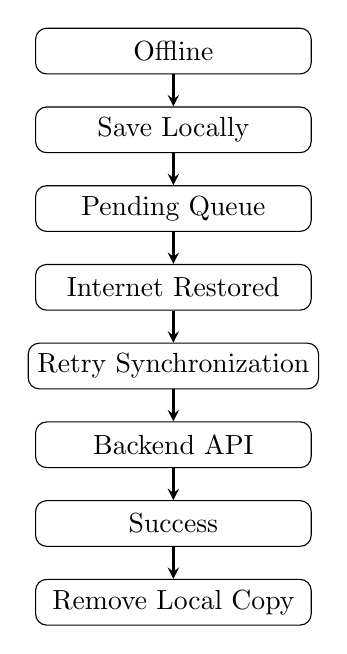
\begin{tikzpicture}[>=stealth,
        syncbox/.style={draw,rounded corners,align=center,minimum width=3.5cm,
                        minimum height=0.58cm}]
        \node[syncbox] (offline) at (0,0) {Offline};
        \node[syncbox] (local) at (0,-1) {Save Locally};
        \node[syncbox] (queue) at (0,-2) {Pending Queue};
        \node[syncbox] (restored) at (0,-3) {Internet Restored};
        \node[syncbox] (retry) at (0,-4) {Retry Synchronization};
        \node[syncbox] (backend) at (0,-5) {Backend API};
        \node[syncbox] (success) at (0,-6) {Success};
        \node[syncbox] (remove) at (0,-7) {Remove Local Copy};

        \draw[->,thick] (offline) -- (local);
        \draw[->,thick] (local) -- (queue);
        \draw[->,thick] (queue) -- (restored);
        \draw[->,thick] (restored) -- (retry);
        \draw[->,thick] (retry) -- (backend);
        \draw[->,thick] (backend) -- (success);
        \draw[->,thick] (success) -- (remove);
    \end{tikzpicture}
    \caption{Offline synchronization flow.}
    \label{fig:offline-synchronization-flow}
\end{figure}

\subsubsection*{Synchronization Principle}

Every synchronized request should include a unique client-generated request
identifier (an \textbf{Idempotency Key}) to prevent duplicate operations caused
by network retries or intermittent connectivity.

The backend stores or recognizes this key and returns the result of the original
operation when the mobile application retries the same request, preventing the
business action from being applied more than once.

\clearpage
\setcounter{section}{11}
\section{Security Approach}

\subsection{Overview}

Security is a fundamental aspect of the Workforce Execution Platform due to the
sensitive nature of construction planning, workforce management, and project
execution data.

The proposed security model follows a layered approach that combines
authentication, authorization, secure communication, auditing, and monitoring
to protect both user identities and operational data.

\subsection{Authentication}

The platform uses JWT (JSON Web Token)-based authentication.

After a successful login, users receive an Access Token and a Refresh Token.
The Access Token is attached to every API request and validated by the backend
before processing any operation.

Expired Access Tokens can be renewed using the Refresh Token without requiring
users to log in again.

This approach provides a stateless authentication mechanism suitable for both
desktop and mobile applications.

\subsection{Authorization}

Authorization combines JWT Authentication, Role-Based Access Control (RBAC),
Scope-Based Authorization, and backend business validation. JWT identifies the
authenticated user, project-specific roles determine the user's permissions,
and scopes restrict access to the authorized Project, Region, or Location.
Backend business validation then enforces operational rules that cannot be
expressed safely as generic database constraints.

Each user may receive roles independently for different Projects. The
\texttt{user\_roles} table includes \texttt{project\_id}, and its composite
unique constraint on \texttt{(user\_id, project\_id, role\_id)} prevents a user
from receiving the same role twice within the same Project. The existing
\texttt{user\_scopes} table continues to define Project, Region, and Location
access.

\begin{figure}[htbp]
    \centering
    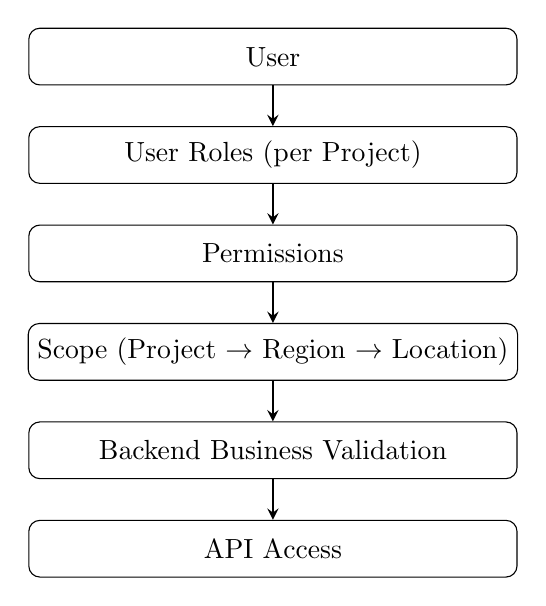
\begin{tikzpicture}[>=stealth,
        authbox/.style={draw,rounded corners,align=center,minimum width=6.2cm,
                        minimum height=0.72cm}]
        \node[authbox] (user) at (0,0) {User};
        \node[authbox] (roles) at (0,-1.25) {User Roles (per Project)};
        \node[authbox] (permissions) at (0,-2.5) {Permissions};
        \node[authbox] (scope) at (0,-3.75)
              {Scope (Project $\rightarrow$ Region $\rightarrow$ Location)};
        \node[authbox] (validation) at (0,-5) {Backend Business Validation};
        \node[authbox] (access) at (0,-6.25) {API Access};

        \draw[->,thick] (user) -- (roles);
        \draw[->,thick] (roles) -- (permissions);
        \draw[->,thick] (permissions) -- (scope);
        \draw[->,thick] (scope) -- (validation);
        \draw[->,thick] (validation) -- (access);
    \end{tikzpicture}
    \caption{Authorization evaluation flow.}
    \label{fig:authorization-evaluation-flow}
\end{figure}

User authorization is validated using the following hierarchical scopes:

\begin{itemize}
    \item Project
    \item Region
    \item Location
\end{itemize}

This ensures that users can only access data belonging to their authorized
organizational units.

A user may be assigned access at the Project, Region, or Location level,
depending on business requirements. Access granted at a higher level applies
to its subordinate organizational units, subject to the user's role and
permissions.

Database constraints prevent duplicate role assignments, while backend
business validation prevents conflicting operational roles. For the MVP, a
user cannot hold multiple operational roles---Head of Master, Site Chief,
Technical Office Engineer, or Project Manager---within the same Project. This
Separation of Duties rule prevents a user from approving their own work.

If a conflicting assignment is attempted, the backend returns
\texttt{409 Conflict} with the reason:

\begin{quote}
\texttt{User already has an operational role in this project.}
\end{quote}

\subsection{Password Security}

User passwords are never stored in plain text.

Passwords are securely hashed using a strong password-hashing algorithm such
as Argon2, with bcrypt available as an alternative. The system also enforces
password-complexity requirements and supports secure password-reset
procedures.

\subsection{API Security}

All communication between clients and the backend is protected using HTTPS.

The backend validates every incoming request through:

\begin{itemize}
    \item JWT verification
    \item Permission checks
    \item Scope validation
    \item Input validation
    \item Request payload validation
\end{itemize}

Standard HTTP status codes are returned for unauthorized or invalid requests.

\subsection{Audit Logging}

To ensure traceability and accountability, all critical business operations are
recorded in an audit history.

Examples include:

\begin{itemize}
    \item Daily Plan creation
    \item Daily Plan modification
    \item Workflow submission
    \item Approval and rejection actions
    \item User login events
\end{itemize}

Each audit record stores:

\begin{itemize}
    \item User
    \item Action
    \item Entity
    \item Timestamp
    \item Previous Status
    \item New Status
\end{itemize}

\begingroup
\scriptsize
\renewcommand{\arraystretch}{1.2}
\setlength{\tabcolsep}{2.5pt}
\begin{tabularx}{\textwidth}{|>{\raggedright\arraybackslash}p{0.14\textwidth}|>{\raggedright\arraybackslash}p{0.10\textwidth}|>{\raggedright\arraybackslash}p{0.10\textwidth}|>{\raggedright\arraybackslash}p{0.12\textwidth}|>{\raggedright\arraybackslash}p{0.11\textwidth}|>{\raggedright\arraybackslash}p{0.11\textwidth}|>{\raggedright\arraybackslash}X|}
    \hline
    \textbf{Timestamp} & \textbf{User} & \textbf{Action} & \textbf{Entity} &
    \textbf{Old Status} & \textbf{New Status} & \textbf{Comment} \\
    \hline
    23 Jul 2026, 10:15 & Site Chief & Approve & Daily Plan DP-1042 & Submitted &
    Site Approved & Work quantities verified. \\
    \hline
    23 Jul 2026, 11:05 & Project Manager & Reject & Daily Plan DP-1048 & Site
    Approved & Rejected & Actual Man-Day requires correction. \\
    \hline
\end{tabularx}
\renewcommand{\arraystretch}{1}
\endgroup

Audit records are immutable and cannot be modified by application users. This
audit trail supports operational transparency and simplifies future
investigations.

\subsection{Logging \& Monitoring}

The platform includes centralized application logging and operational
monitoring.

Application logs capture system events, warnings, and unexpected errors, while
monitoring tools provide visibility into system health and performance.

The minimum operational monitoring coverage is summarized below:

\renewcommand{\arraystretch}{1.15}
\begin{tabularx}{\textwidth}{|>{\raggedright\arraybackslash}p{0.28\textwidth}|>{\raggedright\arraybackslash}X|}
    \hline
    \textbf{Metric} & \textbf{Purpose} \\
    \hline
    API Latency & Measures API response time and highlights degraded request
    performance. \\
    \hline
    Error Rate & Tracks failed requests and unexpected application errors. \\
    \hline
    CPU Usage & Identifies sustained processing pressure on application
    infrastructure. \\
    \hline
    Memory Usage & Detects excessive consumption, resource exhaustion, and
    potential memory leaks. \\
    \hline
    Database Availability & Confirms that PostgreSQL is reachable and able to
    serve application requests. \\
    \hline
    Health Check Endpoint & Exposes application and dependency readiness for
    monitoring and deployment platforms. \\
    \hline
\end{tabularx}
\renewcommand{\arraystretch}{1}

These metrics help identify operational issues and improve system reliability.
Potential technology options include Grafana, Prometheus, the ELK Stack, or
cloud-native monitoring solutions. The architecture remains technology-neutral
so that the most appropriate tooling can be selected for each deployment
environment.

\subsection{Secrets Management}

Sensitive configuration values such as JWT secrets, database credentials, and
API keys are stored outside the application source code using environment
variables or a secure secrets-management solution.

This reduces the risk of credential exposure and simplifies deployment across
different environments.

\subsection{MVP Considerations}

For the MVP, the platform implements the core security mechanisms required for
production use:

\begin{itemize}
    \item JWT Authentication
    \item RBAC Authorization
    \item Organizational Scope Validation
    \item Backend Business Validation for conflicting operational roles
    \item HTTPS Communication
    \item Password Hashing
    \item Audit Logging
    \item Centralized Logging
\end{itemize}

More advanced security features, such as Multi-Factor Authentication (MFA),
Single Sign-On (SSO), and external identity providers, can be introduced in
future releases as business requirements evolve.

\clearpage
\section{Scope Hierarchy (Authorization Scope)}

\begin{figure}[htbp]
    \centering
    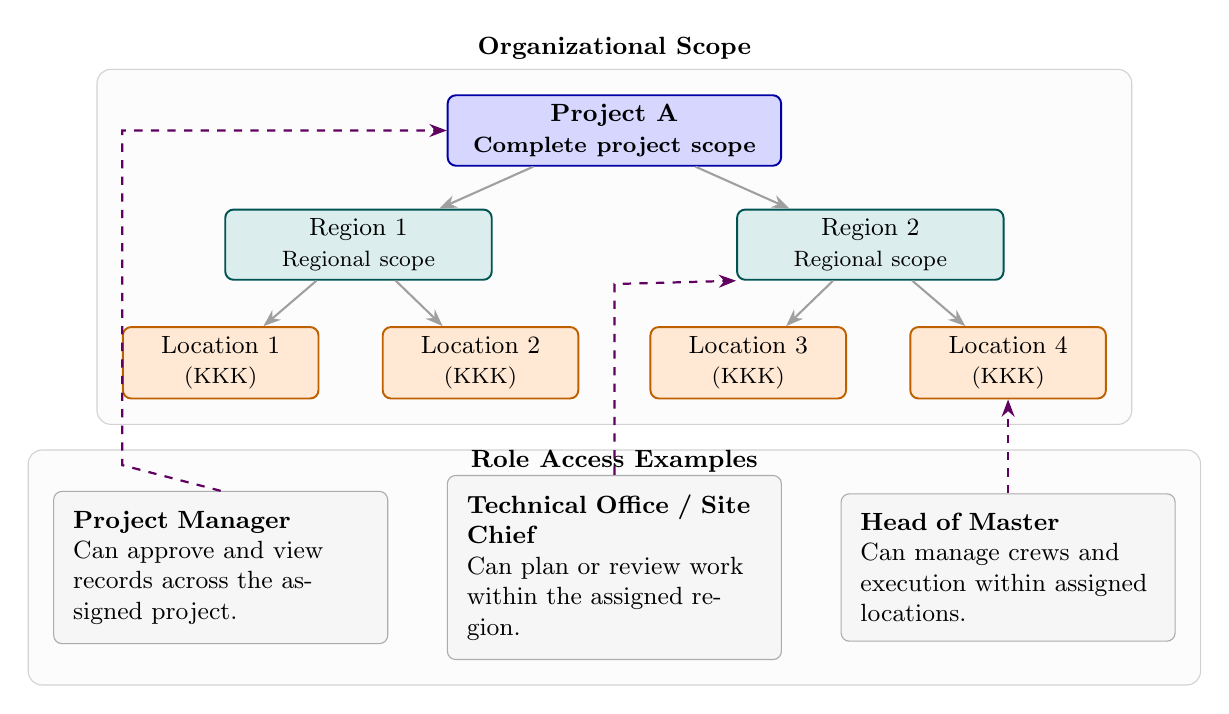
\begin{tikzpicture}[
        font=\small,
        hierarchy/.style={
            draw,
            rounded corners=3pt,
            minimum height=0.85cm,
            align=center,
            line width=0.7pt
        },
        project/.style={
            hierarchy,
            fill=blue!16,
            draw=blue!65!black,
            text width=4.0cm,
            font=\small\bfseries
        },
        region/.style={
            hierarchy,
            fill=teal!14,
            draw=teal!65!black,
            text width=3.15cm
        },
        location/.style={
            hierarchy,
            fill=orange!17,
            draw=orange!75!black,
            text width=2.25cm
        },
        role/.style={
            draw=gray!65,
            rounded corners=3pt,
            fill=gray!7,
            text width=3.75cm,
            minimum height=1.45cm,
            align=left,
            inner sep=7pt
        },
        relation/.style={-{Stealth[length=2.2mm]}, line width=0.75pt,
            draw=gray!75},
        access/.style={-{Stealth[length=2.2mm]}, line width=0.8pt,
            dashed, draw=violet!75!black}
    ]
        % Organizational scope hierarchy
        \node[project] (project) at (0,0)
            {Project A\\\footnotesize Complete project scope};

        \node[region] (region1) at (-3.25,-1.45)
            {Region 1\\\footnotesize Regional scope};
        \node[region] (region2) at (3.25,-1.45)
            {Region 2\\\footnotesize Regional scope};

        \node[location] (loc11) at (-5.0,-2.95)
            {Location 1\\\footnotesize (KKK)};
        \node[location] (loc12) at (-1.7,-2.95)
            {Location 2\\\footnotesize (KKK)};
        \node[location] (loc21) at (1.7,-2.95)
            {Location 3\\\footnotesize (KKK)};
        \node[location] (loc22) at (5.0,-2.95)
            {Location 4\\\footnotesize (KKK)};

        \draw[relation] (project) -- (region1);
        \draw[relation] (project) -- (region2);
        \draw[relation] (region1) -- (loc11);
        \draw[relation] (region1) -- (loc12);
        \draw[relation] (region2) -- (loc21);
        \draw[relation] (region2) -- (loc22);

        % Representative role-to-scope assignments
        \node[role] (pm) at (-5.0,-5.55) {
            \textbf{Project Manager}\\
            Can approve and view records across the assigned project.};
        \node[role] (regional) at (0,-5.55) {
            \textbf{Technical Office / Site Chief}\\
            Can plan or review work within the assigned region.};
        \node[role] (hom) at (5.0,-5.55) {
            \textbf{Head of Master}\\
            Can manage crews and execution within assigned locations.};

        \begin{scope}[on background layer]
            \node[draw=gray!35, rounded corners=5pt, fill=gray!2,
                fit=(project)(region1)(region2)(loc11)(loc12)(loc21)(loc22),
                inner sep=9pt,
                label={[font=\small\bfseries]above:Organizational Scope}] {};
            \node[draw=gray!35, rounded corners=5pt, fill=gray!2,
                fit=(pm)(regional)(hom), inner sep=9pt] {};
        \end{scope}

        \node at (0,-4.20) [font=\small\bfseries]
            {Role Access Examples};

        \draw[access] (pm.north) -- (-6.25,-4.25) |- (project.west);
        \draw[access] (regional.north) -- (0,-3.75) -- (0,-1.95) --
            (region2.south west);
        \draw[access] (hom.north) -- (loc22.south);
    \end{tikzpicture}
    \caption{Scope-based authorization hierarchy and role access examples.}
    \label{fig:scope-authorization-hierarchy}
\end{figure}

The system combines RBAC (Role-Based Access Control) with Scope-Based
Authorization.

RBAC determines \textbf{WHAT} a user can do (permissions).

Scope determines \textbf{WHERE} a user can perform those actions (Project
$\rightarrow$ Region $\rightarrow$ Location).

Every API request validates both the user's permissions and their assigned
scope before granting access.

\clearpage
\section{Technology Stack \& Justification}

\subsection{Overview}

The proposed technology stack prioritizes simplicity, maintainability, and
scalability while supporting the MVP objectives. The selected technologies are
mature, widely adopted, and provide a strong foundation for future platform
growth.

Alternative technologies are also considered to allow flexibility based on
organizational standards or future requirements.

\begingroup
\small
\renewcommand{\arraystretch}{1.2}
\setlength{\tabcolsep}{4pt}
\begin{longtable}{|>{\raggedright\arraybackslash}p{0.15\textwidth}|>{\raggedright\arraybackslash}p{0.19\textwidth}|>{\raggedright\arraybackslash}p{0.18\textwidth}|>{\raggedright\arraybackslash}p{0.38\textwidth}|}
    \hline
    \textbf{Layer} & \textbf{Preferred Technology} & \textbf{Alternative} & \textbf{Justification} \\
    \hline
    \endfirsthead
    \hline
    \textbf{Layer} & \textbf{Preferred Technology} & \textbf{Alternative} & \textbf{Justification} \\
    \hline
    \endhead
    Frontend & React + Next.js & Angular & Component-based architecture,
    strong ecosystem, excellent performance, and reusable UI components. \\
    \hline
    Mobile & React Native & Flutter & Cross-platform development with a
    shared JavaScript/TypeScript ecosystem and faster MVP delivery. \\
    \hline
    Backend & NestJS & Django / ASP.NET Core & Modular architecture,
    dependency injection, TypeScript support, and excellent maintainability
    for enterprise applications. \\
    \hline
    Database & PostgreSQL & Microsoft SQL Server & ACID compliance,
    reliability, advanced indexing, JSON support, and excellent scalability. \\
    \hline
    Cache & Redis & Memcached & Fast in-memory caching for permissions and
    frequently accessed data. \\
    \hline
    Workflow & Application State Machine & Temporal / Camunda & The workflow
    is simple in the MVP and can be managed within the application. External
    workflow engines can be introduced later if business processes become more
    complex. \\
    \hline
    Authentication & JWT + RBAC & OAuth 2.0 / Keycloak & Stateless
    authentication with fine-grained authorization using roles and
    permissions. \\
    \hline
    Notifications & Firebase Cloud Messaging (FCM) & OneSignal & Reliable push
    notifications for mobile users with simple integration. \\
    \hline
    Reporting & Power BI & Grafana & Power BI is already required by the
    business for KPI reporting and dashboards. \\
    \hline
    Deployment & Docker + Kubernetes & Docker Compose & Kubernetes provides
    scalability, self-healing, and streamlined production deployments, while
    Docker Compose is suitable for local development. \\
    \hline
    Monitoring & Prometheus + Grafana & Azure Monitor / Datadog & Provides
    visibility into application health, resource utilization, and performance
    metrics. \\
    \hline
    Logging & ELK Stack & Loki & Centralized log collection and troubleshooting
    across application components. \\
    \hline
\end{longtable}
\renewcommand{\arraystretch}{1}
\endgroup

\subsection{MVP Considerations}

The selected technology stack intentionally avoids unnecessary complexity
during the MVP phase. A modular monolith architecture combined with PostgreSQL,
Redis, and REST APIs provides a solid foundation while allowing future
evolution toward microservices, workflow engines, and event-driven
architectures without significant redesign.

\clearpage
\section{Future Enhancements}

\subsection{Overview}

The proposed MVP architecture provides a solid foundation for future
expansion. While the initial implementation focuses on delivering the core
business workflow, the modular architecture allows new capabilities to be
introduced with minimal impact on the existing system.

Potential future enhancements include the following capabilities.

\subsection{Configurable Workflow Engine}

Replace the application-based workflow with a configurable workflow engine
that allows administrators to define approval steps, transition rules, and
validation logic without modifying the application code.

\subsection{Background Processing}

Introduce message queues and background workers for long-running operations
such as notifications, report generation, external system integrations, and
scheduled tasks.

\subsection{ERP \& HR Integration}

Integrate with existing Enterprise Resource Planning (ERP) and Human Resources
(HR) systems to synchronize employee information, organizational structures,
and project data automatically.

\subsection{Advanced Notification System}

Support multiple notification channels, including:

\begin{itemize}
    \item Push notifications
    \item Email notifications
    \item SMS notifications
\end{itemize}

\subsection{Real-Time Updates}

Introduce WebSocket or SignalR technology to provide real-time updates for
approvals, notifications, and dashboard metrics.

\subsection{Multi-Tenant Architecture}

Extend the platform to support multiple companies or business units while
maintaining complete data isolation between tenants.

\subsection{Advanced Reporting \& Analytics}

Enhance reporting capabilities by introducing predictive analytics, trend
analysis, and AI-assisted productivity insights.

\subsection{Offline Synchronization Improvements}

Support advanced conflict-detection and conflict-resolution strategies for
complex offline scenarios.

\subsection{Fine-Grained Workflow Configuration}

Allow administrators to configure approval chains, validation rules,
permissions, and business policies without requiring an application
deployment.

\clearpage
\section{Conclusion}

The proposed solution delivers a scalable and maintainable Workforce Execution
Platform that satisfies the core business requirements while following the
Minimum Viable Product (MVP) approach.

The architecture adopts a modular monolith design with clear separation of
responsibilities, enabling rapid development, simplified deployment, and
straightforward maintenance. Core business capabilities---including daily
planning, crew management, approval workflows, reporting, and
notifications---are implemented as independent modules, allowing future
evolution without significant architectural changes.

The proposed technology stack combines proven enterprise technologies such as
PostgreSQL, Redis, JWT-based authentication, RESTful APIs, and Power BI to
provide a reliable, secure, and extensible solution.

By prioritizing simplicity in the MVP while designing for future scalability,
the platform establishes a strong foundation for upcoming enhancements such as
configurable workflows, ERP and HR integration, real-time communication,
multi-tenant operation, and advanced analytics.

\end{document}
